\section{Analytical Modeling Of MPI Applications}
\label{sec-model}

To effectively reduce the overhead of network communications in MPI
applications, one must understand when and where it becomes beneficial
to enhance the overlap of communications with local computations in
these applications. Through an analytical approach, our
framework aims to model the runtime execution flow of an input
application in terms of its relative amount of time spent in local
computations and network communications.  This information then is
used to automatically identify potential communication bottlenecks as
candidates for optimization in the later steps.

To represent and estimate the time required to execute the local computation of
each path, we use the \texttt{Bayesian Execution Tree} (\texttt{BET})
from the Skope analytical performance modeling
framework~\cite{jichi:ipdps14}.  Each BET essentially represents
possible runtime code paths of an application together with their
execution frequency and expected execution time. We use the Skope
framework to automatically generate a BET representation of each
application from the application source code combined with some sample
input data and code-coverage profiling of the application execution.
We then extend the Skope framework to additionally estimate the
overhead of each MPI communication through the following steps.

\begin{enumerate}

\item Use a LogGP-based communication model for the MPI runtime to
  estimate the communication time for each individual MPI call.

\item Statistically estimate the expected average communication time
  for each code path by combining the individual communication with
  the execution frequencies.

\end{enumerate}

Finally, the balance between the time required for each MPI communication and
the expected execution time of its surrounding local computation is
used to project optimization opportunities. The following first
illustrates the BET representation that we inherit
from~\cite{jichi:ipdps14} and then explains our extensions for
modeling MPI communications.


\subsection {Bayesian Execution Tree}

\begin{figure}[h]
\begin{center}
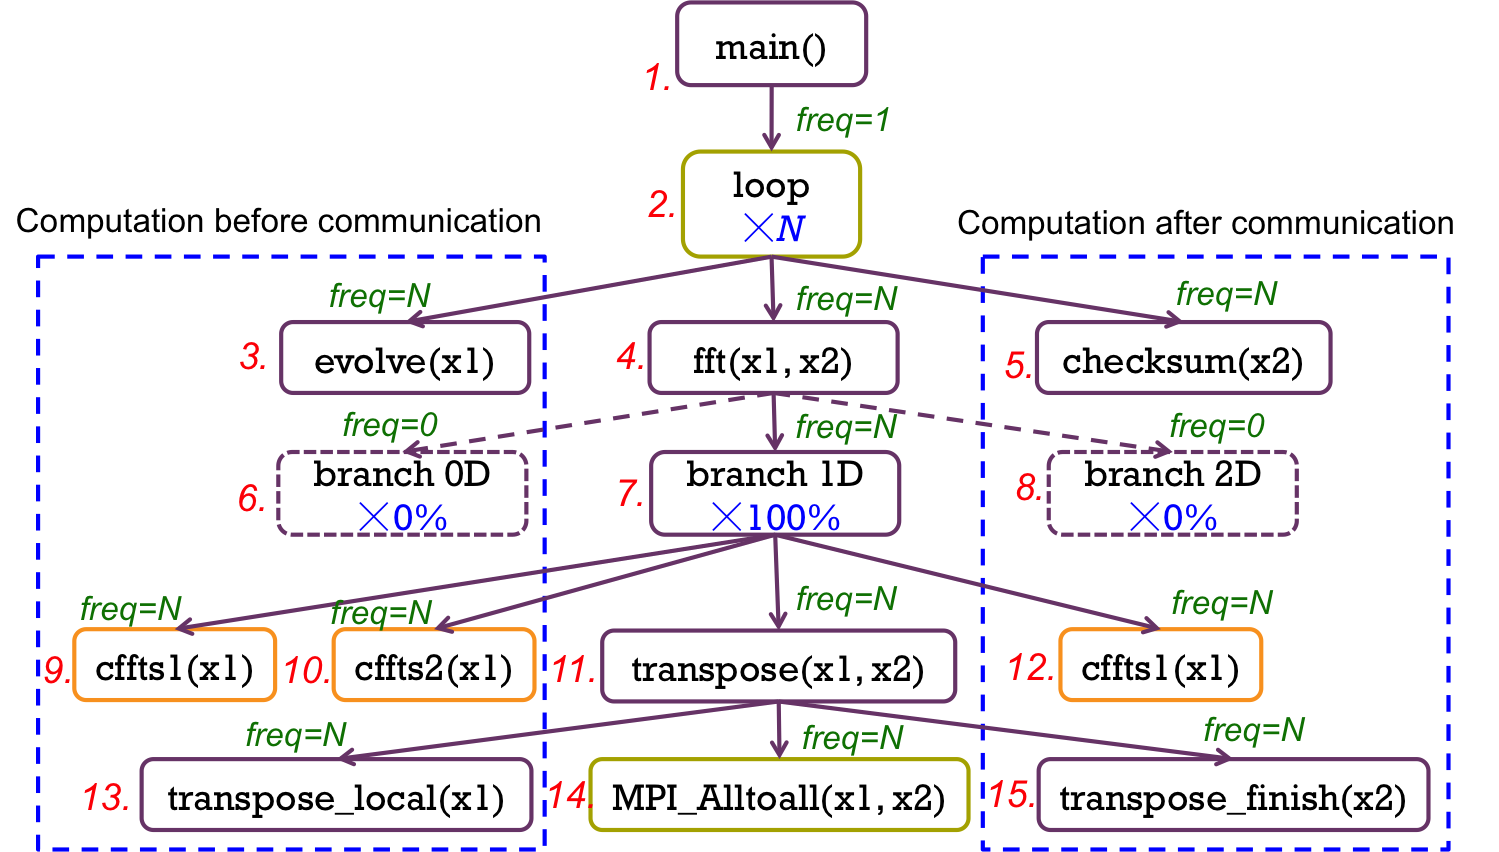
\includegraphics[width=0.48\textwidth]{fig/ft_bet.png}
\caption{Simplified Bayesian Execution Tree for NAS 1D FFT before
  overlapping computation and communications \emph{(only important branches, loops, and function calls are shown})}
%, and not all nodes and frequencies in BET are drawn in this figure)}}
\label{fig:ft_bet}
\end{center}
\end{figure}

Figure~\ref{fig:ft_bet} shows an example \texttt{BET} for one of the
MPI processes of the NAS FT benchmark in Figure~\ref{fig:ft_loop}.
Each node of the BET represents a code block (a sequence of statements
in the user program) together with its \emph{runtime execution
  frequency}, defined as the expected average number of times that
statements in the code block will be executed at runtime.  A
\texttt{depth-first-traversal} (\texttt{DFS}) of each subtree of the
\texttt{BET} corresponds to a possible runtime execution path of the
statements.  For example, in Figure~\ref{fig:ft_bet}, Node\#2 is a
loop of $N$ iterations, so the frequency of its loop body is $N$.
Node\#7 is a branch inside the {\em fft} function. If the application is
to perform 1D FFT, this branch is taken 100\% of time during
execution, so its frequency is $N$, while the frequency of the
alternative branches (Node\#6 and Node\#8) are set to 0.

In order to derive execution frequencies of each code block, the Skope
framework requires a description of the application input data,
manually provided by the user or in our case,  automatically collected via 
instrumented runs of the application.  The input data description
characterizes the possible values of data that the application
may obtain from external sources, for example, command-line arguments,
environment variables, or files.  For array variables, only their
dimensions and the size of each dimension are required.  For MPI
applications, the total number of MPI processes
(\texttt{MPI\_Comm\_size}) and the rank of the process to model
(\texttt{MPI\_Rank}) are additionally required.  Based on the input
data description, the Skope framework applies constant propagation to
derive possible values of the expressions that control the directions
of branch and loop controls. A fall-through probability is assumed to be 50\% if the values cannot be accurately determined.  For this
paper, we used \texttt{gcov} to profile applications with sample input
data,


\subsection{Modeling MPI Communications}

To predict MPI communication overhead, we have extended the Skope framework with the LogGP
model~\cite{loggp} to additionally model the latency (elapsed time) of
each MPI operation using the following four parameters:

\begin{enumerate}

\item $P$: number of processes involved in the communication

\item $n$: size (in bytes) of the message being transferred

\item $alpha$: overhead of starting each message and time interval
  required between transmitting each pair of messages

\item $beta$: communication time per byte for large messages,
  determined by the underlying network bandwidth.

\end{enumerate}

Among the four parameters, $alpha$ and $beta$ can be calculated  ahead of time from
characteristics of the underlying network. We compute
$beta$ as the reciprocal of the network bandwidth and $alpha$ by using
microbenchmarks to measure the latency of \texttt{MPI\_Send} and
\texttt{MPI\_Recv} operations on the target platform.  The other two
parameters, $P$ and $n$, are determined through instrumented
runs of the user application.
% or obtained directly from the user as expected runtime configurations of the application.  
In particular,
$P$ equals to \texttt{MPI\_Comm\_size}; and $n$ 
is obtained from the values used to invoke the MPI operations.

Following the LogGP model, we model the cost (latency) of each MPI point-to-point communication
as:

\begin{equation}
cost_{p2p}(n;alpha,beta) = alpha + n\cdot beta .
\end{equation}

To model the \texttt{MPI\_Alltoall} operation, we use the following two
formulas.

\begin{equation}
  cost_{short} = log P\cdot alpha + \frac{n}{2}\cdot log P\cdot beta
\end{equation}

\begin{equation}
cost_{long} = (P-1)\cdot alpha + n\cdot beta
\end{equation}

The first formula models the latency of short messages and
the second that of long messages.  We use values of \emph{control
  variables} from the MPI runtime library, for example,
\texttt{MPIR\_CVAR\_ALLTOALL\_SHORT\_MSG\_SIZE} for MPI alltoall, to
determine whether a message should be categorized as {\em short} or
{\em long} and thereby select the proper formulas to use.

After estimating the latency of each individual MPI operation,
the overall communication time of a code path in BET can be calculated
by adding the communication time of all code blocks along the path,
using the following formula.

\begin{equation}
  cost_{m} = \sum\limits_{i}^{m} cost(i) * freq(i)
\end{equation}

Specifically, the total communication time of a path of $m$ nodes in
the BET can be computed as the sum of the latency of each
individual MPI operation multiplied by its execution frequency
$freq(i)$.  Here, $freq(i)$ is calculated as the same of the frequency of the BET node that contains the MPI operation, and
$cost(i)$ is calculated as indicated above using LogGP formulas
instantiated with the expected parameter values of the MPI operations.
For example, the total communication time of \texttt{MPI\_Alltoall} in
Figure~\ref{fig:ft_bet} can be computed by multiplying the average
communication time of \texttt{MPI\_Alltoall} by the number of
iterations of the loop node\#2 ($\times N$) and the fall-through
probability of the 1D FFT branch node\#7 ($\times 100\%$).
